\documentclass{beamer}
\usepackage{graphicx}

\usetheme{Copenhagen}
\usecolortheme{beaver}

% hide navigation butons at bottom
\setbeamertemplate{navigation symbols}{}

\title{Übertragung von Signalen auf elektrischen Leitungen}
\author{Sven Schmidt}


\begin{document}

% Title page with image at the top
\begin{frame}
    \centering
    % Insert and center the image at the top
    
\includegraphics[width=0.5\textwidth]{logo_fernuni_hagen.png}
    \vspace{0.5cm} % Adjust space between image and title as needed

    {\LARGE \textbf{\inserttitle}}\\[0.5cm]

    \textbf{Proseminar Mathematik in der Technik}\\
    \textbf{Modulnummer:} 61711\\
    Fakultät für Mathematik + Informatik\\[0.5cm]

    \begin{tabbing}
        \hspace{4cm} \= \kill
        \textbf{Name:} \> Sven Schmidt \\
        \textbf{Matrikelnummer:} \> 4125169 \\
        \textbf{Prüfer:} \> PD Dr.-Ing. Stefan Helfert \\
    \end{tabbing}

    \vfill

    {\large FernUniversität in Hagen}\\
    {\large Sommersemester 2025}
\end{frame}


\section{Herleitung der Telegraphenleitung}


\begin{frame}{Modell des Zweidrahtleiters}

Wir betrachten ausschließlich Paralleldrahtleiter.

\begin{figure}[!htb]
    \begin{center}
        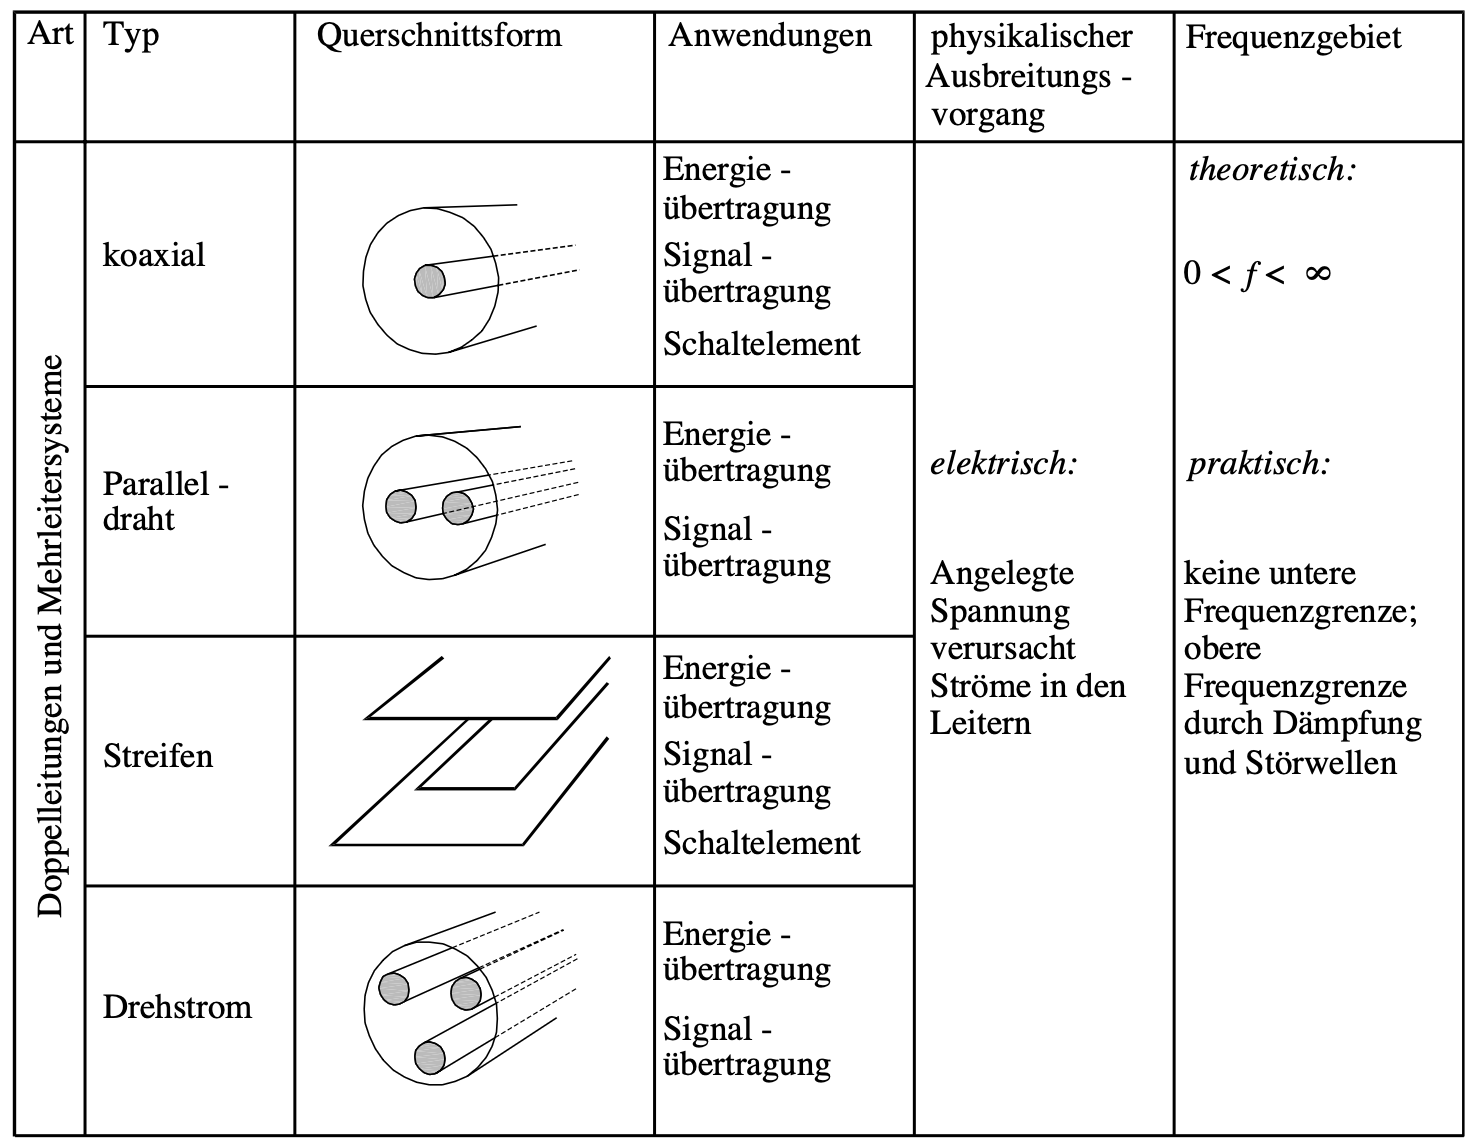
\includegraphics[width=0.75\textwidth]{../Ausarbeitung/images/Leiter.png}
    \end{center}
\end{figure}

\end{frame}


\begin{frame}{Leitungsbeläge}

Ein Leitungsstück der Länge $s$:
\begin{figure}[!htb]
    \begin{center}
        \includegraphics[width=0.5\textwidth]{graphics/Ersatzschaltbild4/document}
    \end{center}
\end{figure}





\end{frame}


\end{document}
